%% ee149.tex
%% V0.1
%% 2012/11/30
%%
%% http://www.ctan.org/tex-archive/macros/latex/contrib/supported/IEEEtran/
%%

% *** Authors should verify (and, if needed, correct) their LaTeX system  ***
% *** with the testflow diagnostic prior to trusting their LaTeX platform ***
% *** with production work. IEEE's font choices can trigger bugs that do  ***
% *** not appear when using other class files.                            ***
% Testflow can be obtained at:
% http://www.ctan.org/tex-archive/macros/latex/contrib/supported/IEEEtran/testflow

\documentclass[conference, 10pt]{IEEEtran}

% some very useful LaTeX packages include:

\usepackage{cite}
\usepackage{graphicx}
\graphicspath{{./Figures/}}
\DeclareGraphicsExtensions{.png, .pdf}
\usepackage{url}
\usepackage{amsmath}
\usepackage{listings}
\lstset{language=C, basicstyle=\ttfamily\footnotesize, numbers=none, numberstyle=\tiny, tabsize=4, showstringspaces=false}

% correct bad hyphenation here


\begin{document}

% paper title
\title{Marauder's Map -- Achieving Semantic Indoor Localization for Smartphones using Ultrasound}

% author names and affiliations
% use a multiple column layout for up to three different
% affiliations
\author{\IEEEauthorblockN{Ben Zhang}
\IEEEauthorblockA{EECS Department\\
University of California, Berkeley\\
Berkeley, CA 94720\\
E-mail: \url{benzh@eecs.berkeley.edu}}
\and
\IEEEauthorblockN{Hokeun Kim}
\IEEEauthorblockA{EECS Department\\
University of California, Berkeley\\
Berkeley, CA 94720\\
E-mail: \url{hokeunkim@eecs.berkeley.edu}}
\and
\IEEEauthorblockN{Zachary Hargreaves }
\IEEEauthorblockA{EECS Department\\
University of California, Berkeley\\
Berkeley, CA 94704\\
E-mail: \url{hargreaves.z@berkeley.edu}}
}

% make the title area
\maketitle

\begin{abstract}
Indoor localization has been studied for a long time due to a considerable number of applications' requirement. While the ability of providing precise geo-location is important, researches have identified that most applications only require semantic location.

In this paper, we propose the semantic localization concept, and demonstrate its effectiveness. To achieve it, we also designed and implemented an ultrasound-based indoor localization system (named Marauder's Map), which could tell the semantic location of a smartphone holder.
\end{abstract}

%%%%%%%%%%%%%%%%%%%%%%%%%%%%%%%%%%%%%%%%%%
\section{Introduction}
\label{sec:introduction}

While Global Positioning System (GPS)~\cite{hofmann1993global} has been extensively relied on recently for many applications such as navigation, geo-tagging, etc, it doesn't work well for indoor environment due to the block of line-of-sight to satellites. Various approaches have been investigated to achieve precise indoor localization, and a sizable number of those researches are trying to localize specific devices or sensor nodes, and many have associate these ``tags'' with human to achieve location-based services. 

Such investigation gets another wave of attention after the emerging smartphones which act naturally as everyone's tag. Though limited by types of sensors, most smartphones are equipped with cellular, Wifi, Bluetooth, inertial measurement unit (IMU), microphone, camera, speaker, etc. Lastest smartphones may even support near field communication (NFC), Bluetooth Low Energy (BLE), proximity sensor, light sensor and even barometer. These sensors have make smartphones not only primarily for communication, but also become such embedded programming platform that many researchers can fast prototype and deploy systems to a large amount of users. And among them are the indoor localization systems.

Although a fair amount of them are concentrating on providing precise 3D coordinates as the localization results (mainly relying on the RF signal attenuation and triangulation), recently focus has been shifted to address room-level detection as the localization results. This change has been mainly inspired from the requirements of many applications, but has converted the localization problem to a classification problem, where the main challenge is to find the proper signature/feature to assist the classifier.

However, most existing signatures (Cellular, Wifi, FM, Acoustic Background Sound), are not precise to provide high accuracy of detection. In this project, we propose that it's easy to create reliable man-made signature of each room with little infrastructure installation -- by deploying ultrasound beacons in each room could provide such signature. And the best part of this approach is the utilization of the ultrasound signal reflection inside each room. Another great benefit is the pervasive existence of microphone on smartphones. Since we do not require any distance information being calculated, no synchronization or sophiscated encoding scheme is needed. The entire system is fairly simple yet effective.

We will detail our design and implementation in this paper with the structure as follows. Related indoor localization investigation will be discussed in Sec.\,\ref{sec:related-works}. And in Sec.\,\ref{sec:system-architecture}, we focus on the design of the system architecture. The implementation details are in Sec.\,\ref{sec:implementation}, which is followed by the evaluation in Sec.\,\ref{sec:evaluation}. Potential future work lies in Sec.\,\ref{sec:future-work} and Sec.\,\ref{sec:conclusion} concludes this paper.

%% Master
%%% Local Variables: 
%%% mode: latex
%%% TeX-master: "ee149"
%%% End: 

\section{Related Works}
\label{sec:related-works}

Localization problems have been widely researched because location information of people, vehicles or any type of moving targets can be useful for providing the target's behavior, availability, safety and so on. Localizing targets outdoors has become relatively easier thanks to the technologies such as (GPS). Indoor localization problems, however, are still under research from various viewpoints. Early investigations include the Active Badge~\cite{want1992active} system uses wearable infrared transmitters. And there were many approaches using wireless signals to achieve indoor localization (see the survey paper in \cite{liu2007}). These wireless signals include cell phone signals such as cellular~\cite{otsason2005accurate} that are most common in daily life nowadays, which have advantages in the sense that this method does not demand any additional equipment for localization. Swangmuang and Krishnamurthy~\cite{Swangmuang2008} conducted research on indoor localization technique using fingerprint based positioning with wireless signals. FM~\cite{chen2012fm} signals, with its pervasiveness, could also be leveraged to achieve localization. There has also been research carried out using an active RFID tag~\cite{Jin2006, buettner2009recognizing}.

Semantic indoor localization, which is useful for providing information, not as exact coordinates of a target, but as which part of space the target is located, is what we have undertaken in this project. We divided an environment where we process indoor localization into semantic places such as offices, laboratories, seminar rooms or sections in a convention center and localize targets and provide this information for users. This kind of semantic place classification was dealt with in Rottmann's work~\cite{rottmann2005semantic}. In this respect, we chose ultrasonic signals, which can be easily blocked by walls or cubicles that divide an environment into semantic spaces, to convey the location information as beacon signals. There has been research using ultrasound signals for indoor localization with ultrasonic sensors~\cite{feng1997mobile, priyantha2005cricket}, which is closely related to our project, although they used ultrasounds to measure distance with the method of triangulation rather than carry information as we did in this project.



%%% Local Variables: 
%%% mode: latex
%%% TeX-master: "ee149"
%%% End: 


\section{System Architecture}
\label{sec:system-architecture}

We will talk about system architecture in this chapter, and reason about its design.

%% Master
%%% Local Variables: 
%%% mode: latex
%%% TeX-master: "ee149"
%%% End: 

% the folder implementation contains 
% ultrasound, android, backend related tex file
\section{Implementation}
\label{sec:implementation}

In this section, we will describe our approaches separately to each component of this system. 

\subsection{Ultrasound Beacons}
\label{sec:ultrasound-beacons}


	Commercially viable ultrasound beacons were designed to minimize consumer cost while maintaining easy portability.  While adhering to these design specifications inherent system constraints were introduced. Creating a low powered solution reliant on battery power was ideal due to portability requirements.  The ultrasound nodes were initially designed for room level localization requiring cell phone microphones to detect audio emissions from 0 -10 meters away from the beacons. After receiving data from the beacons a fast Fourier transformation was computed to determine the frequency content of the signal received.  The fast Fourier transformation requires a precise sinusoidal input for interference not to occur in frequencies in close proximity with the initially generated frequency.  

	With all of these design constraints considered an Atmega328p was used to generate digital sinusoidal signals, this digital output was processed by a DAC, smoothed with a Chebyshev filter, and then amplified.  
 
\begin{figure}[h]
  \centering
  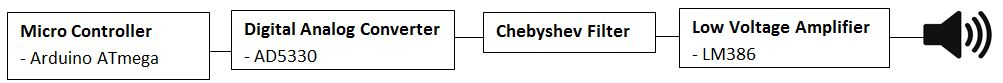
\includegraphics[width=\columnwidth]{ultrasound_design.png}
  \caption{Ultrasound Generator System Architecture}
  \label{fig:ultrasound_design}
\end{figure}

	In order to generate samples at a consistent rate an interrupt service routine synced with the Atmega’s internal 16MHz clock was implemented. With this high sample rate,  generating precise frequencies was feasible but bottle necked by the interrupt service routine's (ISR) execution time resulting in repetition of sample values until execution was completed  (Fig 3). The execution time for the ISR was directly dependent on the method used to set digital output values. The DigitalWrite() method provided in the Arduino library is an abstraction created to make ease of use for users, unfortunately this abstraction adds overhead and resulted in a 24 microsecond execution time whereas writing to registers directly reduced execution time significantly bringing it down to 5 microsecond.  

	In order to smooth out the voltage plateaus caused by the ISR a low pass filter was introduced (Fig 3). A Chebyshev low pass filter with a cut off frequency of 17 kHz performed optimally to generate a more precise/smooth output.  Once filtered the signal was at a fine enough resolution for FFT operations to be performed with no noise/interference in unwanted frequencies.  The output from the filter yielded a 2 Volt signal with about 20 mA of current so amplification was needed in order to drive the 0.5 Watt speaker. 

\begin{figure}[h]
  \centering
  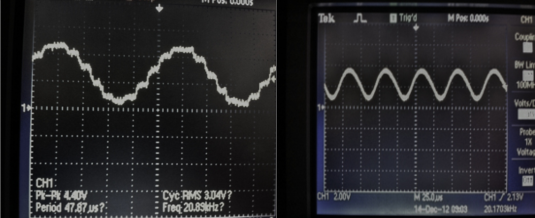
\includegraphics[width=\columnwidth]{filter_effect.png}
  \caption{Left: ISR execution time created notable steps in the digital output 
		Right: Smoothing after the signal was processed by the Chebyshev filter}
  \label{fig:filter_effect}
\end{figure}

	The LM386 power amplifier was ideal due to the low power constraints of the project.  Upon implementation it was immediately apparent the amplifier was not performing to manufacturing specifications making the output challenging to debug. Other amplifiers were implemented but required too much supply voltage ($>$ 9 Volts) to be feasible candidates for the project.  Due to time limitations amplification was not properly achieved but amplification to the required specifications is certainly attainable. 




%% Master
%%% Local Variables: 
%%% mode: latex
%%% TeX-master: "ee149"
%%% End: 

\subsection{Android Application}
\label{sec:android-application}

The main role of the Android application in this system is to receive ultrasonic waves using microphones on the smartphones. Therefore, the ultrasonic signal range is required to satisfy two conditions. The signal should not be heard by humans, at the same time it should be heard by microphones. The audible range of frequency for humans is between 20Hz and 20kHz, while most microphones on smartphones support sampling rate of 44.1kHz, which is greater than Nyquist rate relative to the highest human audible frequency, 40kHz, to avoid aliasing of the signal. However, as 44.1 kHz is still higher than the Nyquist rate, we can easily speculate that the smartphones are theoretically capable of recording the frequency range between 0 Hz to 22.05 kHz without aliasing, although it will become more difficult to differentiate signals when the frequency gets closer to either of two extremes. The frequency band ranging from 20 kHz to 22.05 kHz satisfies the two conditions mentioned above; this band is not hearable for humans but still hearable for smartphones. However, according to our experiments, the received signal strength becomes too weak to be feasible around the frequency of 21.0 kHz when the frequency goes higher.

The amount of computation gets overly intensive when the number of points in fast Fourier transform (FFT) exceeds 2048. Although the more number of points in FFT gives us the finer granularity to represent data using ultrasound signals, increasing the number of points in FFT requires more computations, which can be a burden for embedded systems such as smartphones. After carrying out experiments related to the proper number of points in FFT, we concluded that 2048 points would be a limit for current smartphones since 4096 point FFT slightly slowed down the response time of recent Android devices like Samsung GalaxyS 3 and Google Nexus 7. 2048 point FFT gives us a feasible resolution of approximately 10.76 Hz per each point so we have about 94 points from 20.0 kHz to 21.0 kHz. It is not possible to fully utilize these points as bits because there is noise in FFT results around the target frequencies due to limitation of precision in sound generation and FFT. Considering the interference caused by neighboring signals, leaving space in frequencies between signals would be proper to obtain clear data from decoding. Therefore, we divided this range of frequency between 20.0 kHz and 21.0 kHz into eight intervals removing 21.0 kHz frequency from the range in order to increase correctness in decoding, assigning 8 bits at between 20.0 kHz and 20.875 kHz as demonstrated in Fig.\,\ref{fig:data_representation}.

<<<<<<< HEAD
To decode room ID from FFT results, differentiating the actual signal value from noise and interference caused by ultrasound generators, environments and neighboring signals. Before taking interference by neighboring signals into consideration, the noise by the generator should be eliminated. Even though the created wav signal by Matlab is quite clear, it might involve some noise from speakers and circuits. If the application always try to choose the FFT result at the exact target frequency it will still have chances to select a signal weaker than what is actually necessary for decoding as shown in Fig. \ref{fig:fft_results} box (a). Selecting maximum value among the results which are right beside to the target frequency rather than just picking up the value at the exact frequency can remove this possibility, and we call this value as a “signal value”. The easiest way to detect a signal is to compare the signal value with an absolute value and determine that there is a signal if the signal value is greater than absolute value. However, this method does not work because the signal at neighboring frequencies will affect the FFT result of the target frequency making it hard to differentiate the real signal and the fake signals caused by noise of neighboring signals such as in Fig. \ref{fig:fft_results} box (b). To differentiate actual signals from noise and interference of neighboring signals, just comparing the signal value with an absolute value is not sufficient. This tricky problem can be solve by setting “reference values” to be compared with the signal value. Even though there is noise by the signals around
the signal value, they tend to be diminished as they get further
from its target frequency. Hence, if the signal value is greater
than FFT results around the signal value, then we can conclude
that there is a signal. The reference values are set as the sum
of the FFT results apart from the target frequency by three
points scaled by a predefined factor and a base noise, which is
a threshold or an absolute value that is set according the target
frequency. Since the received signal strength becomes weaker
as the frequency increases, the threshold is set to decrease as
the target frequency increases.
=======
To decode room ID from FFT results, differentiating the actual signal value from noise and interference caused by ultrasound generators, environments and neighboring signals. Before taking interference by neighboring signals into consideration, the noise by the generator should be eliminated. Even though the created wav signal by Matlab is quite clear, it might involve some noise from speakers and circuits. If the application always try to choose the FFT result at the exact target frequency it will still have chances to select a signal weaker than what is actually necessary for decoding as shown in Fig.\,\ref{fig:fft_results} box (a). Selecting maximum value among the results which are right beside to the target frequency rather than just picking up the value at the exact frequency can remove this possibility, and we call this value as a “signal value”. The easiest way to detect a signal is to compare the signal value with an absolute value and determine that there is a signal if the signal value is greater than absolute value. However, this method does not work because the signal at neighboring frequencies will affect the FFT result of the target frequency making it hard to differentiate the real signal and the fake signals caused by noise of neighboring signals such as in Fig.\,\ref{fig:fft_results} box (b). To differentiate actual signals from noise and interference of neighboring signals, just comparing the signal value with an absolute value is not sufficient. This tricky problem can be solve by setting “reference values” to be compared with the signal value. Even though there is noise by the signals around the signal value, they tend to be diminished as they get further from its target frequency. Hence, if the signal value is greater than FFT results around the signal value, then we can conclude that there is a signal. The reference values are set as the sum of the FFT results apart from the target frequency by three points scaled by a predefined factor and a base noise, which is a threshold or an absolute value that is set according the target frequency. Since the received signal strength becomes weaker as the frequency increases, the threshold is set to decrease as the target frequency increases.
>>>>>>> 8163bf77635d1f6a94fe4156c1dba2436042dae3

The Android application is able to determine whether there is a signal by comparing the signal value to the reference values as explained above. But there is one more problem left that needs a solution, the decoded value using this method is still unstable changing frequently as time passes. This can lead to wrong reading or too frequent fluctuation of room ID that makes it difficult to localize the target.  The problem can happen especially when the target person with a phone enters a room with an ultrasound generator. The application employs an exponential moving average denoted in \ref{eqn:1} to stabilize the decoded result and wait until the decoded value after the exponential moving average becomes constant to avoid frequent fluctuation when the localization process begins right after the target enters a room with an ultrasound generator.

\begin{equation}
t>1, s_t=\alpha \cdot y_t+(1-\alpha)\cdot s_{t-1}
\label{eqn:1}
\end{equation}
By using this two-level filtering method, we could obtain almost perfectly clear room ID results.
\ref{eqn:1}

This application also provides additional features to show the target's location depending on the user's selection. Users can choose to share their position on a map through the sMAP server using HTTP POST by sending the localization result to a dedicated server. By setting the user's name on the application interface, the users can publish their positions on the map provide by the server so that other people can identify where they are. The users may keep their location information secret without publishing their position to the public for their privacy. In this case, the application uses a map embedded to the application to show the location of the target without specifying the user's name. The user interface of Android application is also illustrated in Fig.\,\ref{fig:app_interface}. The space between check boxes and a start/stop button can be used to show either the private map or FFT results in graph as shown in leftbottom of the Fig.\,\ref{fig:app_interface}.

\begin{figure}
  \centering
  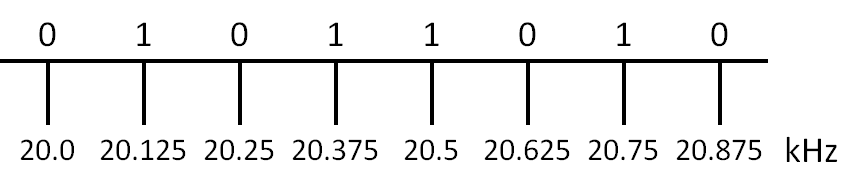
\includegraphics[width=0.8\columnwidth]{data_representation.png}
  \caption{Data representation on frequency band ranging from 20.0 kHz to 20.875 kHz}
  \label{fig:data_representation}
\end{figure}

\begin{figure}
  \centering
  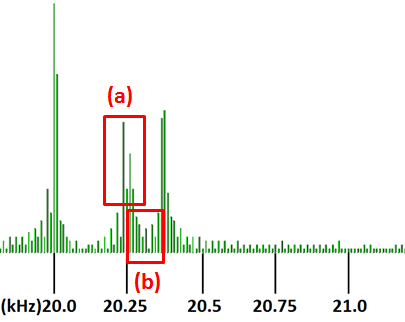
\includegraphics[width=0.7\columnwidth]{fft_results.png}
  \caption{Results of 2048 point FFT on Android application}
  \label{fig:fft_results}
\end{figure}

\begin{figure}
  \centering
  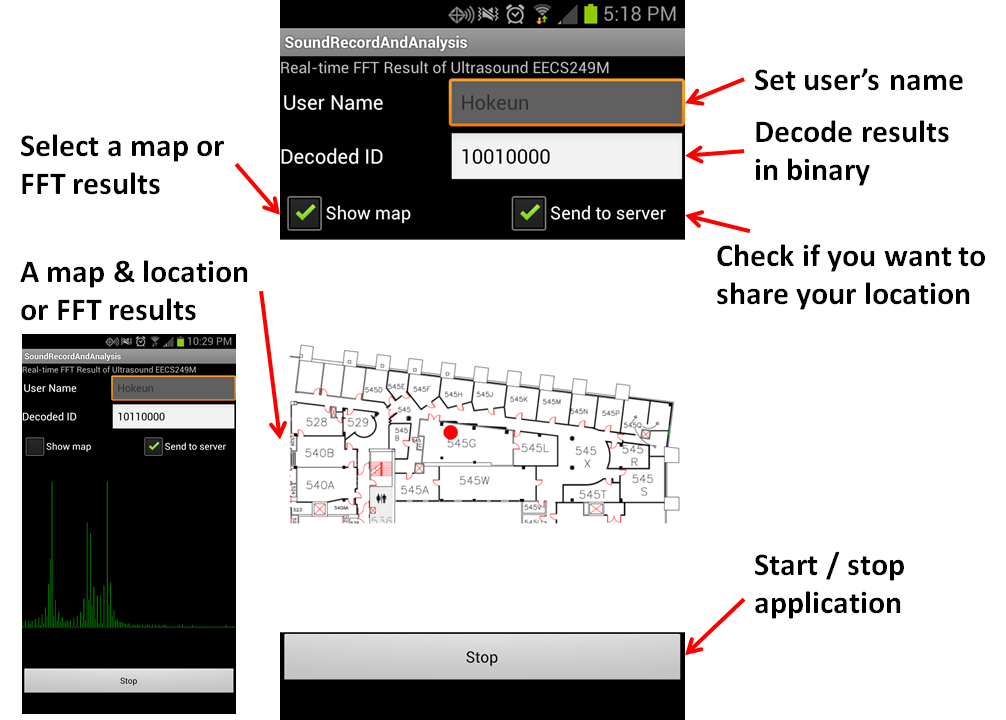
\includegraphics[width=\columnwidth]{app_interface.png}
  \caption{User interface of Anrdoid application}
  \label{fig:app_interface}
\end{figure}

%% Master
%%% Local Variables: 
%%% mode: latex
%%% TeX-master: "ee149"
%%% End: 

\subsection{Backend Aggregator}
\label{sec:backend-aggregator}

Ben should talk about the implementation of the backend server and front end html page.

%% Master
%%% Local Variables: 
%%% mode: latex
%%% TeX-master: "ee149"
%%% End: 

%% Master
%%% Local Variables: 
%%% mode: latex
%%% TeX-master: "ee149"
%%% End: 


\section{Evaluation}
\label{sec:evaluation}

In this section, we performed several experiments to characterize such an ultrasound localization system.

\subsection{Power Consumption}
\label{sec:power-consumption}
We have measured the power consumption of our application on LG Revolution VS910 with Android 2.3.4. The summarized measured results are in Table.\,\ref{tab:power}. We could easily found out that having this application running in the background doesn't affect much of the power consumption. While having the application running in front, since there are a lot of screen drawings on the UI update event (either display the spectrum or the map), the application apparently burdens the battery (with an increase of about 59.8\% power consumption than usual).

Since there are so many factors which could potentially influence the power consumption, the measurement is mostly for some rough estimation. But one interesting thing that we do observe by measuring the power consumption is that, most power is used for screen, and more than 100mA current is usually used for radio and communication (there is occasional peaks when the screen is off). 

\begin{table}
  \centering
  \begin{tabular}{|l|c|c|}
    \hline
    & mean (mA) & standard variance (mA) \\
    \hline
    no app, screen on &  214.9 & 43.6 \\
    no app, screen off &  72.4 & 48.0 \\
    \hline
    app runs, screen on &  342.0 & 43.6 \\
    app runs {\em (background)}, screen on & 211.0 & 10.0 \\
    app runs {\em (background)}, screen off &  56.5 & 49.5 \\
    \hline
  \end{tabular}
  \caption{Power consumption of the application}
  \label{tab:power}
\end{table}


% screen on mean: 0.2149 var: 0.0019 -> 0.0436
% screen off mean: 0.0724 var: 0.0023 -> 0.0480
% % Screen on: 0.3256 0.1948 0.3563 0.2035 0.2110 0.1878 0.1874 0.1867 0.2207 0.2261 0.2135 0.2041 0.2014 0.1888 0.1893 0.1888 0.1882 0.1897 0.1913 0.1873 0.2036 0.1968 0.2691 0.2453 lab
% % Dim: 0.1854
% % Screen off: 0.0818 0.0318 0.0099 0.0833 0.0497 0.0062 
% % 0.0051 0.0037 0.0050 0.0041 0.0071 0.1202 0.1035 0.1232 0.0060 0.0052 0.1046 0.0905 0.0317 0.1014 0.0909 0.1588 0.1700 0.0836 0.0965 0.0924 0.1064 0.0568 0.0951 0.0900 0.0766 0.1246 0.0900 0.1034 0.0145 0.0059 0.0550 0.0451 0.0898 0.1050

% Running application
% screen on mean: 0.3420 var: 0.0027 -> 0.0520 
% screen on background mean: 0.2110 var: 0.0001 -> 0.01
% screen off background mean: 0.0565 var: 0.0024 -> 0.0495
% % Screen on: 0.2248 0.2379  0.2325     0.3312 0.3529 0.3512 0.3686 0.3519 0.4118 0.3416 0.3504 0.3339 0.3298 0.3499 0.3162 0.3495 0.3649 0.3471 0.3269 0.3626 0.3561  0.3585 0.3570 0.3495 0.3355 0.3749 0.3629 0.2559 0.4544 0.3623 0.3545 0.4343 0.4395 0.3946 0.3798 0.3525 0.3433 0.3490 0.3696 0.3338 0.3635 0.3433 0.3695 0.3141 0.3861 0.3173 0.3707 0.3736 0.4577 0.3371 0.3577 0.3421 0.3356 0.3393 0.3387 0.3484 0.3566 0.3178 0.3536 0.3573 0.3297 0.3238 0.2341 0.2349 0.2621 0.3493 0.3477 0.3499 0.3412 0.3438 0.3565 0.3502 0.3403 0.3599 0.3514 0.3402 0.3530 0.3416 0.3330 0.3690 0.3484 0.3600 0.2275 0.2181 0.2460 0.2364 0.2379 0.2623 0.3735 0.3502 0.4430 0.4042 0.4276 0.4293 0.3523 0.3373 0.3593 0.3107 0.3767 0.4200 0.3066 0.2086  
% % background screen on
% 0.2136 0.1883 0.2018 0.1941 0.1909 0.1907 0.1880 0.1924 0.1881 0.2056 0.1877 0.2001 0.2554 0.2251 0.2787 0.2756 
% % background screen off
% 0.0769 0.0649 0.0698 0.1014 0.0225 0.0077 0.0047 0.0045 0.0127 0.0043 0.0041 0.0350 0.1009 0.1676 0.0726 0.1196 0.0905 


\subsection{Signal Strength}
\label{sec:signal-strength}
We measure the received siganl strength using commercial laptop (Macbook Pro). The maximum output sound level is 86$\sim$90dB. Since we have converted the received signal to frequency domain, the results are only relative values for the purpose of illustration of ultrasound's characteristics. The obtained figure is shown in Fig.\,\ref{fig:strength}, where we measured four different frequency point, ranging from 20 inches to 140 inches. We conducted our experiment in Room 545K, whose length is around 150 inches. 

This figure shows that generally the received ultrasound signal is attenuating with the increasing of distances. There might exist several points where the received signal strength is larger than those who are nearer; this is mainly caused by all kinds of reflection inside this room. Another observation is that with the increase of signal frequency, the signal strength is descreasing due to the imperfect frequency response of most microphones used in smartphones, but these several signals are still large enough to be differetiated from the nosie.

\begin{figure}
  \centering
  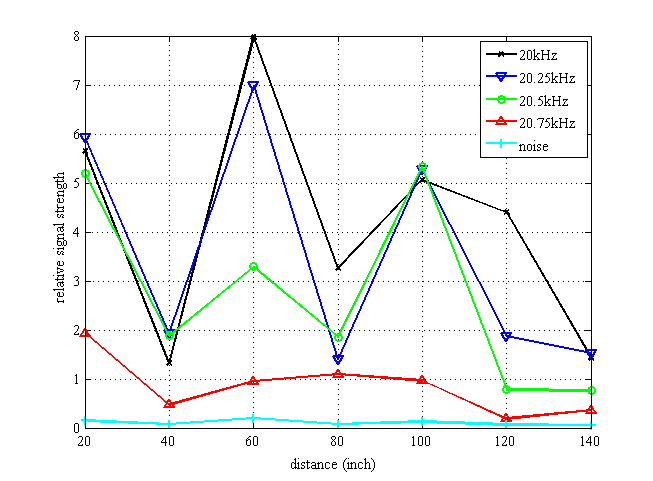
\includegraphics[width=0.9\columnwidth]{result_distance.png}
  \caption{Signal Strength vs. Distance}
  \vspace{-0.3cm}
  \label{fig:strength}
\end{figure}

\subsection{Obstacle Blocking}
\label{sec:obstacle-blocking}
As we have argued in Sec.\,\ref{sec:introduction} that the ultrasound can be easily reflected inside a room while the wall can be perfect deliminator of spaces. In this section, we describes the experiment of validating such idea by measuring both the signal strength and the detection rate. We place the phone on both side of the glass wall of Room 545K, and run this application both for more than 1 minute. 

The measurement of received signal after FFT operation is shown in Fig.\,\ref{fig:wallblock}. It's clearly attenuated after the blocking of the wall. We then calculate the detected results (the groundtruth in this case is 10110000), the ``inside'' experiment can mostly correctly detect the room ID, with an accuracy of 96.06\% (it's 91.25\% before the filtering) while the ``outside'' experiment always outputs 0.

\begin{figure}
  \centering
  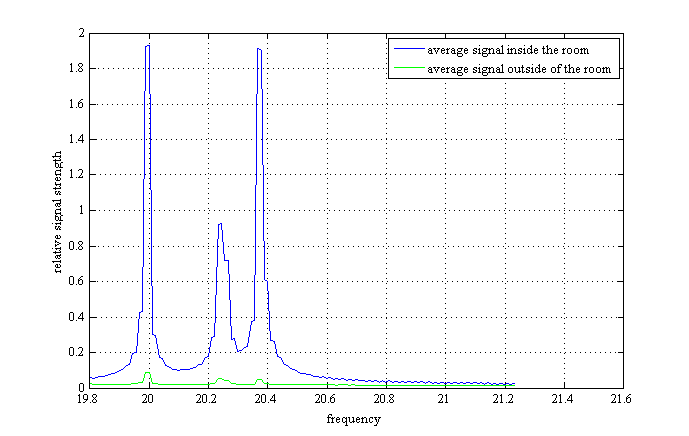
\includegraphics[width=0.9\columnwidth]{WallBlocking}
  \vspace{-0.3cm}
  \caption{The effect of wall blocking}
  \label{fig:wallblock}
\end{figure}

\subsection{Room Coverage}
\label{sec:room-coverage}
In last section, we examined the effect of walls which will block the signal easily, and therefore the signal should be bouncing back and forth inside the room to create a fully coverage. We did experiment about such coverage characteristics but measuring eight different points inside the room. We compare the detected results with the groundtruth (both before and after filtering) and draw the related accuracy in Fig.\,\ref{fig:coverage}. And from the result we could easily see that the ultrasound signal covers the entire room, and works pretty well for corner-cases. 
\begin{figure}
  \centering
  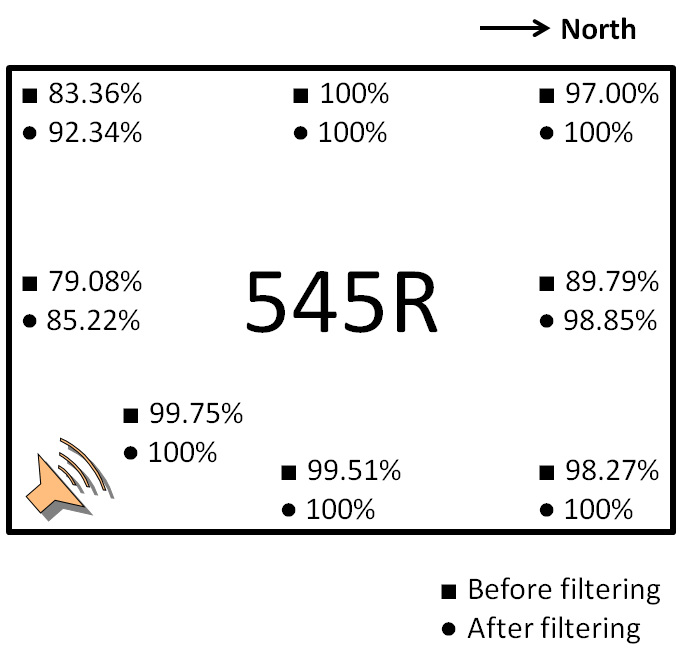
\includegraphics[width=0.6\columnwidth]{545R.png}
  \vspace{-0.3cm}
  \caption{Room coverage experiment}
  \label{fig:coverage}
\end{figure}

\subsection{Noise Resistance}
\label{sec:noise-resistance}
Another great feature we utilize about ultrasound is its noise resistence. Since talking, playing music and walking will not generate much signal that exceed 20kHz, such an ultrasound-based beacon should be able to resist noise pretty well. In order validate such idea of noise resistence, we need to know how it performs with the existence of different kinds of noise (such as speaking, coughing, music, etc.). 

The experiment result is shown in Table.\,\ref{tab:noiseres}, and it's clear that most human activity won't affect the detection too much. Clapping does affect this since they contains high frequency signals. But this will only affect a lot when clapping is continued for a long time, otherwise such noise will be removed by the exponential averaging filter.
\begin{table}
  \centering
  \begin{tabular}{|l|c|c|}
    \hline
    noise source & accuracy (before filtering) & accuracy (after filtering) \\
    \hline
    speaking &  99.93\% & 100\% \\
    music  &  94.44\% & 100\% \\
    coughing & 97.25\% & 100\% \\
    clapping & 69.17\% & 74.58\% \\
    walking & 100\% & 100\% \\
    \hline
  \end{tabular}
  \caption{Noise resistence characteristics}
  \label{tab:noiseres}
\end{table}

\subsection{Reception Rate}
\label{sec:reception-rate}
In this experiement, we plan to examine the overall detection of our algorithm. Since there are multipath effect, other kinds of noises, the data reception rate will not be perfect. Our exponential moving average algorithm (in Sec.\,\ref{sec:android-application}) is used to cope with these imperfections, and some effect has been shown in previous experiments.

We run our application for 2 mins continously to collect the raw detected results and the filtered results in the normal environment (phone holder moves around naturally during this experiment). The result is shown in Fig.\,\ref{fig:reception}, where we cluster the detected results using the histogram to illustrage the errors. The groundtruth room ID is 176, where the signal is successfully detected most of the time. Bit errors do happen occasionally; from our experiment, the overall reception rate is 67.60\%. After the filtering, some sporadic errors are corrected, and the overall detection has been improved to 87.50\%. 

Further observation reveals that most of the wrong detection resulted in Room ID 0, which means no reliable signal at all. We could just infer users' location as previous room since it's not physically feasible of changing room drastically; such semantic combination with real scenario will yield 97.25\% accuracy.

\begin{figure}
  \centering
  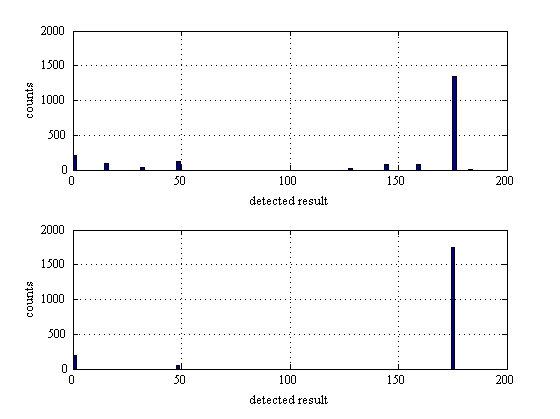
\includegraphics[width=0.9\columnwidth]{ReceptionRate}
  \caption{Histogram of the raw detected room ID ({\em up}); histogram of filtered result ({\em down})}
  \vspace{-0.3cm}
  \label{fig:reception}
\end{figure}




%% Master
%%% Local Variables: 
%%% mode: latex
%%% TeX-master: "ee149"
%%% End: 


\section{Future Work}
\label{sec:future-work}

What may possibly be done afterwards?

%% Master
%%% Local Variables: 
%%% mode: latex
%%% TeX-master: "ee149"
%%% End: 
\section{Conclusion}
\label{sec:conclusion}

The main goal of this project was to implement a feasible semantic indoor localization system that can be used to locate a user's position on a map who is carrying a smartphone so that the person does not need any additional device. Producing information of the semantic spaces was realized by using an ultrasound signal generator that generates sinusoids with specific frequencies and the sinusoids conveyed IDs of rooms in the environment. An Android application was implemented in order to collect audio samples to be decoded into room information using Fast Fourier Transform (FFT) and a couple of filtering algorithms. Calculated location information could be either sent to a server that can aggregate multiple targets' location or kept secret for the user's privacy. This main goal of the project was mostly achieved throughout this semester and we illustrated how accurate and efficient this localization system is by various kinds of experiments. Power consumption caused by this Android application imposed mild overhead on the smartphone, this system showed clear and accurate results even though when there was noise and interference. Through additional evaluation such as tests for room coverage and obstacle blocking, we also proved this system is proper for indoor characteristics. 

%% Master
%%% Local Variables: 
%%% mode: latex
%%% TeX-master: "ee149"
%%% End: 


%% template to put figure
% Layers figure
% \begin{figure}[t]
%   \includegraphics[width=\linewidth]{figFileName}
%   \caption{This is the caption of this figure.}
%   \label{fig:label}
% \end{figure}

%%%%%%%%%%%%%%%%%%%%%%%%%%%%%%%%%%%%%%%%%%

% use section* for acknowledgement
\section*{Acknowledgment}
To begin with, we would like to give thanks to Professor Edward A. Lee and Professor Sanjit A. Seshia for teaching and guiding us to finish this course and course project successfully. We also thank our GSI, Zach Wasson for helping us to learn practical knowledge through labs and giving us feedback and our project mentor, Tomi Räty for leading and giving us advice on the direction of this project.

% references section
% NOTE: BibTeX documentation can be easily obtained at:
% http://www.ctan.org/tex-archive/biblio/bibtex/contrib/doc/

% can use a bibliography generated by BibTeX as a .bbl file
% standard IEEE bibliography style from:
% http://www.ctan.org/tex-archive/macros/latex/contrib/supported/IEEEtran/bibtex
\bibliographystyle{IEEEtran}
% argument is your BibTeX string definitions and bibliography database(s)
%\bibliography{IEEEabrv,../bib/paper}
%
% <OR> manually copy in the resultant .bbl file
% set second argument of \begin to the number of references
% (used to reserve space for the reference number labels box)
%\bibliographystyle{jponewurl}
\bibliography{Refs}
%%%%%%%%%%%%%%%%%%%%%%%%%%%%%%%%%%%%%%%%%%%%%%%%%%%%%%%%%%%%%%%%
%%%%%% NOTE: I didn't delete the origin entries in Refs.bib %%%%
%%%%%% to give us a flavor of format of bibtex (Ben)        %%%%
%%%%%%%%%%%%%%%%%%%%%%%%%%%%%%%%%%%%%%%%%%%%%%%%%%%%%%%%%%%%%%%%

\appendix

\subsection{Role Played in the Project}
\label{sec:role-played-project}
% each member's role in one paragraph
Ben Zhang working on Backend server.
Hokeun Kim has mostly worked on developing the Android application, implementing Fast Fourier Transform (FFT) on collected audio samples, decoding of location information from the FFT results on ultrasonic signals and two-level filtering algorithms to stabilize decoded results. He also designed the user interface of Android application.
Zachary Hargreaves primarily developed the hardware for the ultrasound beacon.  This task required constuction of code to generate a digital sine wave then processing of the signal in order to be compatable with the ultra sound reciever.   

\subsection{Related with EE149 Course}
\label{sec:related-with-ee149}
\subsubsection{Key concepts learned from class}
\label{sec:key-concepts-learned}

Interfacing with sensors (microphone) and understanding the imperfect nature of sensor signals proved valuable when filtering high frequency disturbances in our signals.  The filtering methods introduced in the first lab were directly related to the processing required in our project.  Learnig low-level uC programming was useful when decoding the data sheets in order to understand the role each register played in implementing the ISR.  System modeling helped us avoid future probelems before implementing our network protocol.

\subsubsection{Course feedback}
\label{sec:course-feedback}
Pretty good course. Having more hardware components around the lab would help many projects out. This would streamline the debugging process and encourage cross group collaboration because many groups using similar (class provided) components would be able to help one another out.  

\subsubsection{Technical Challenges}
\label{sec:technical-challenges}
Aside from the bottle necks caused by delivery times for specialized components, understanding amplification circuits for low powered systems was a large technical challenge.
For decoding location information from ultrasounds, coping with noise and interference caused by environments and signal itself was the biggest technical challenge. To deal with varying signal strength according to frequency range and distance from the ultrasound generator was another challenge for developing the Android application.
TODO
 - Noise and interference for the signal   
- stable server 

%% Master
%%% Local Variables: 
%%% mode: latex
%%% TeX-master: "ee149"
%%% End:


\end{document}